\documentclass[11pt]{article}
\usepackage[english]{babel}
\usepackage{amsmath,amssymb,amsfonts}
\usepackage{fullpage}
\usepackage{hyperref}
\usepackage{float}
\usepackage{xcolor}
\usepackage{booktabs}
\usepackage{graphicx}
\usepackage{listings}
\usepackage{titlesec}
\usepackage{fvextra}
% Disable paragraph indentation
\setlength{\parindent}{0pt}%
\setlength{\parskip}{\baselineskip}%
\titleformat{\section}{\large\bfseries}{\thesection}{1em}{}

\lstset{
  language=Python,                 % Set language to Python
  basicstyle=\ttfamily\footnotesize, % Set font and size
  keywordstyle=\color{blue},       % Keywords in blue
  stringstyle=\color{red},         % Strings in red
  commentstyle=\color{green!50!black}, % Comments in green
  backgroundcolor=\color{yellow!10}, % Light gray background
  frame=single,                    % Frame around the code
  numbers=left,                    % Line numbers on the left
  numberstyle=\tiny\color{gray},   % Style for line numbers
  tabsize=6,                       % Set tab width
  showstringspaces=false,           % Hide whitespace symbols
  captionpos=b                     % Caption at the bottom
}

\begin{document}
\title{Assignment3 - DD2424}
\author{Silpa Soni Nallacheruvu}
\date{\today}
\maketitle

\section*{Gradient Check}

To verify the correctness of my analytical gradient computations for my three-layer ConvNet, I implemented a comparison against the provided debug data for the gradients and other available variables. The relative mean and max errors were computed for each layer's weights, biases and more:
\begin{table}[h!]
  \centering
  \begin{tabular}{|l|c|c|}
  \hline
  \textbf{Comparison} & \textbf{Max Difference} & \textbf{Mean Difference} \\
  \hline
  X\_conv Vs conv\_outputs           & $0.0$                        & $0.0$ \\
  conv\_outputs\_mat Vs conv\_outputs\_flat & $1.70 \times 10^{-13}$       & $6.83 \times 10^{-16}$ \\
  conv\_flat                         & $0.0$                        & $0.0$  \\
  h                                  & $0.0$                        & $0.0$  \\
  p                                  & $6.76 \times 10^{-16}$       & $5.01 \times 10^{-17}$ \\
  Fs\_flat                           & $1.64 \times 10^{-14}$       & $8.45 \times 10^{-16}$ \\
  W1                                 & $4.50 \times 10^{-14}$       & $2.03 \times 10^{-16}$ \\
  W2                                 & $4.51 \times 10^{-15}$       & $1.25 \times 10^{-16}$ \\
  b1                                 & $4.22 \times 10^{-16}$       & $4.22 \times 10^{-17}$ \\
  b2                                 & $1.31 \times 10^{-15}$       & $2.34 \times 10^{-16}$ \\
  \hline
  \end{tabular}
  \caption{Numerical comparison of intermediate computations and gradients.}
  \end{table}

As the relative mean and max difference between provided debug values and my computed values are insignificant, I conclude that my implementation is bug free.

\section*{Initial Three layer ConvNet}

The initial three-layer ConvNet was implemented with the following architecture:
\begin{itemize}
  \item Convolutional layer with 32 filters of size 3x3, stride 1, and padding 1.
  \item ReLU activation function.
  \item Max pooling layer with a pool size of 2x2 and stride 2.
  \item Fully connected layer with 128 units.
  \item ReLU activation function.
  \item Output layer with softmax activation for classification.
\end{itemize}

The network was trained on the CIFAR-10 dataset with training size of 49,000 images and validation size of 1,000 images. The short training runs with cyclic learning rates from Assignment2 was applied with a minimum learning rate of 1e-5 and a maximum learning rate of 1e-1 for three cycles with constant steps of 800, and L2 regularization $\lambda = 0.003$.

The intial model with Network architecture 2 ($f=4, nf=10, nh=50$) achieved a final validation accuracy of $56.1\%$ and test accuracy of $55.88\%$. The training time was reported as $13.07$ seconds.

Next, we compare the final test accuracy and training time of the following four network architectures with varying f anf nf values with short training runs:

\begin{itemize}
  \item Architecture 1: $f=2, nf=3, nh=50$
  \item Architecture 2: $f=4, nf=10, nh=50$
  \item Architecture 3: $f=8, nf=40, nh=50$
  \item Architecture 4: $f=16, nf=160, nh=50$
\end{itemize}

\begin{figure}[H]
    \centering
    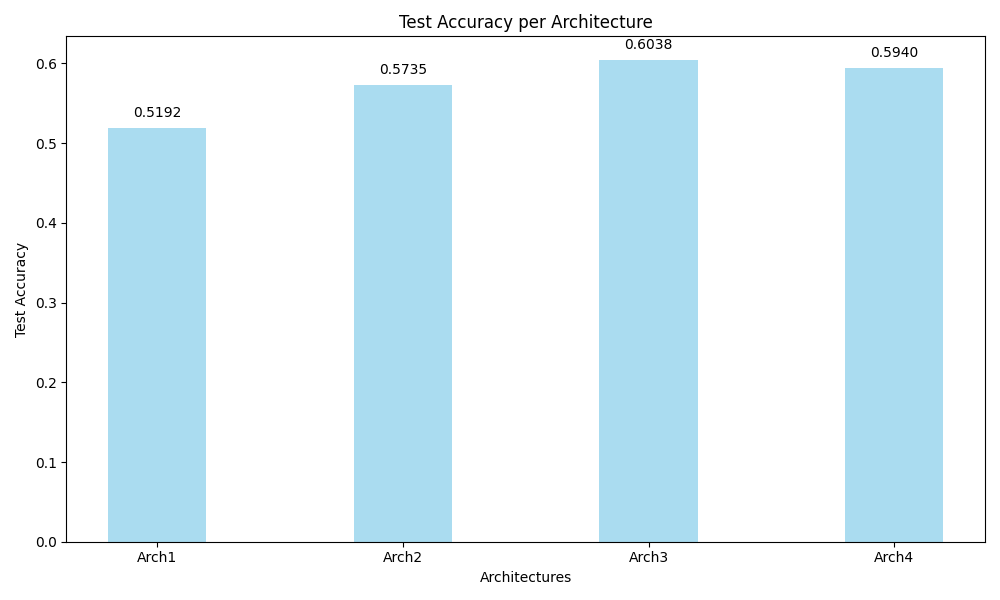
\includegraphics[width=0.7\textwidth]{results/architecture_test_accuracy.png}
    \caption{Comparison of final test accuracy for different network architectures.}
    \label{fig:network_architecture_acc_comparison}
\end{figure}

\begin{figure}[H]
  \centering
  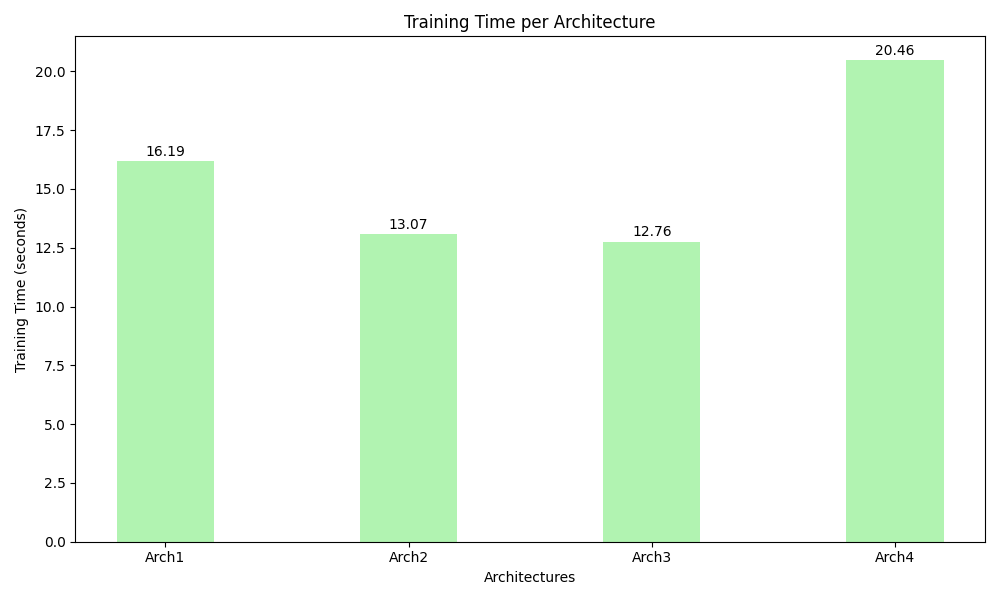
\includegraphics[width=0.7\textwidth]{results/architecture_training_time.png}
  \caption{Comparison of total training time for different network architectures.}
  \label{fig:network_architecture_training_time_comparison}
\end{figure}

The above results show that the test accuracy increases and training time decreases from Arch1 to Arch3 because increasing patch size and filters improves feature extraction and reduces computation (fewer patches per image).
Arch4 gets slower and less accurate because patches become too large, losing spatial info, and the network's dense layers become very large, slowing down training and hurting generalization.

We can conclude that Arch2 and Arch3 are the best performing architectures, with Arch3 being the most efficient in terms of training time and accuracy.

I was able to verify the correctness of the above cyclic learning rate schedule with learning rate curve shown below:

\begin{figure}[H]
    \centering
    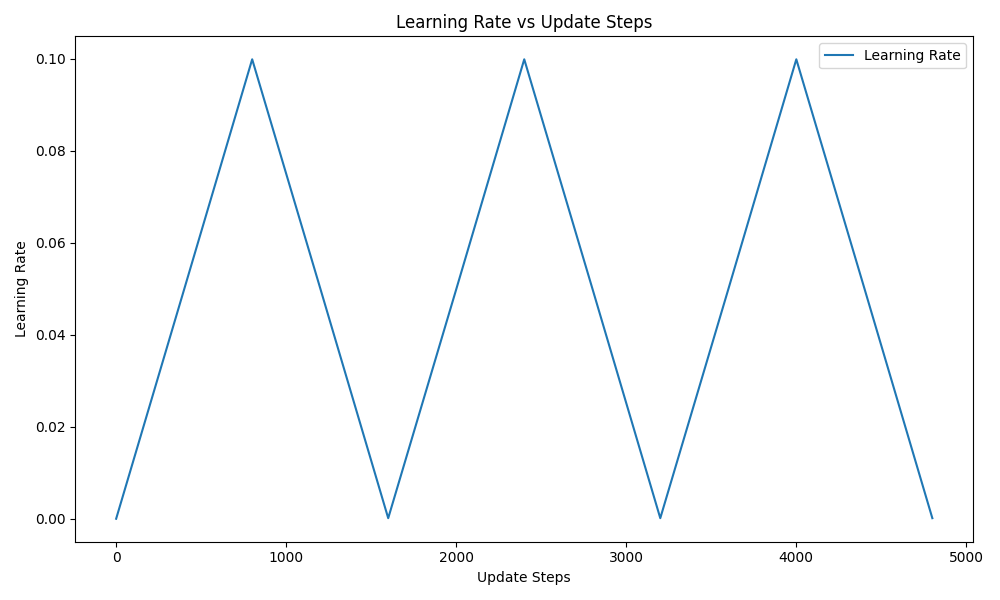
\includegraphics[width=0.6\textwidth]{results/architecture_basic_2_learning_rate_plot.png}
    \caption{Cyclic learning rate schedule for the training runs.}
    \label{fig:cyclic_learning_rate}
\end{figure}

\section*{Longer Training Runs}

Here, we implement the cyclical learning rates with increasing step sizes for longer training runs. The step size is doubled after each cycle, starting from 800 steps. The minimum learning rate is set to 1e-5 and the maximum learning rate is set to 1e-1. The training runs are performed for 3 cycles with the previously mentioned best two architectures, i.e., Network Architecture 2 and 3. The dataset was split into 49,000 training images and 1,000 validation images.
The curves for training Vs validation loss and accuracies is shown below, logged at every $n_s/2$ steps, where $n_s$ is the number of steps in the current cycle.

\begin{figure}[H]
  \centering
  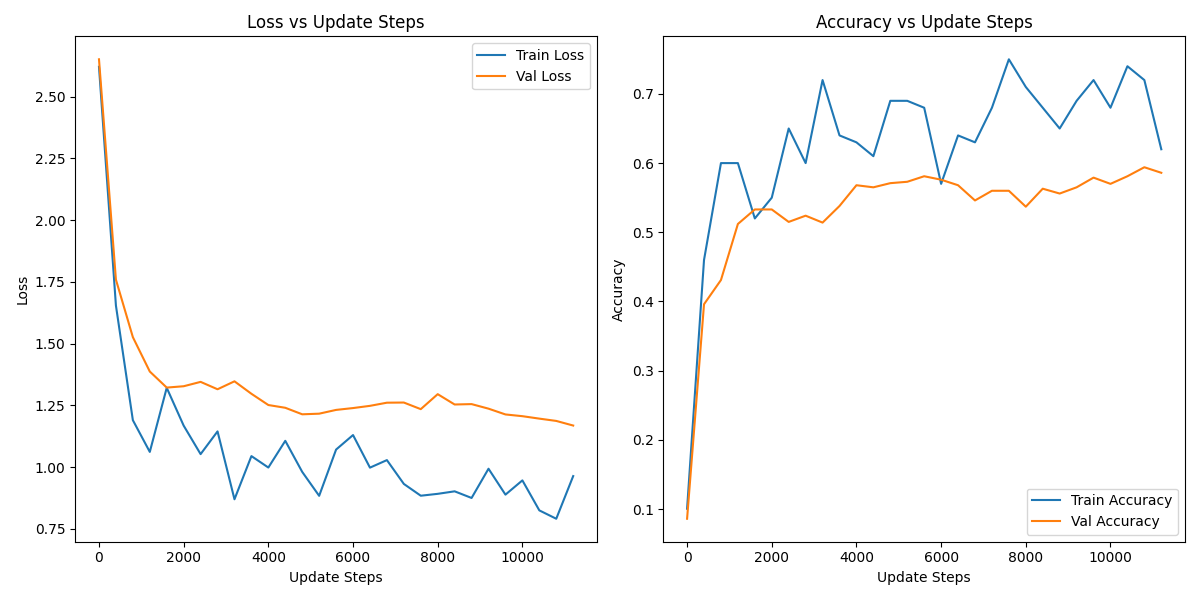
\includegraphics[width=0.75\textwidth]{results/architecture_2_training_plot.png}
  \caption{Training and validation loss and accuracies for longer training runs for the Network Architecture 2 ($f=4, nf=10, nh=50$).}
  \label{fig:longer_training_runs_arch2}
\end{figure}


\begin{figure}[H]
  \centering
  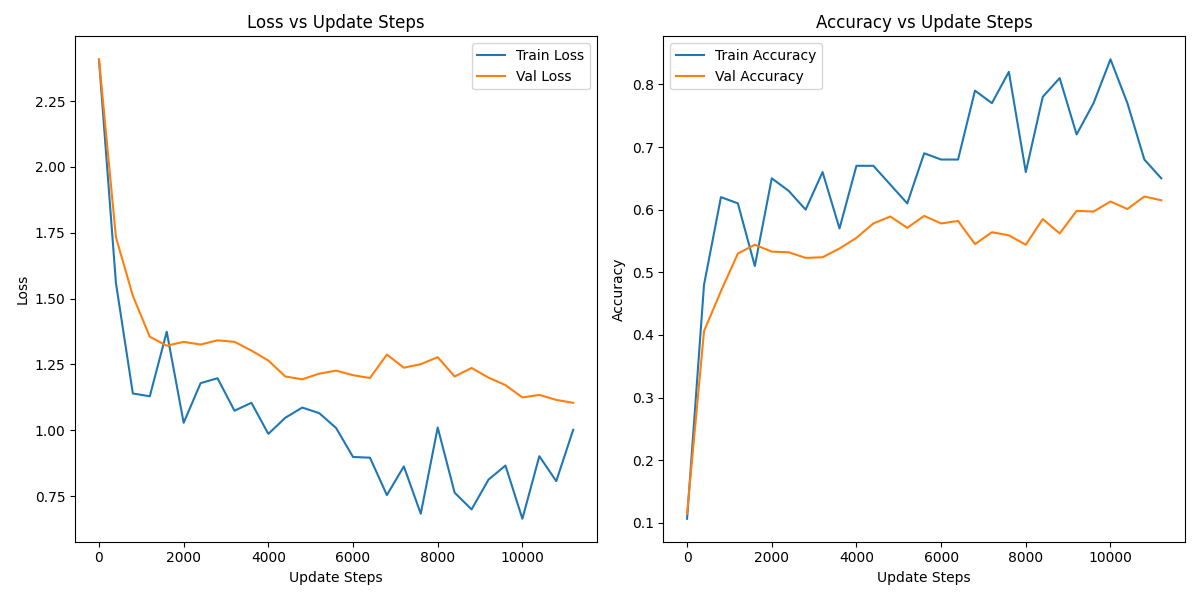
\includegraphics[width=0.75\textwidth]{results/architecture_3_training_plot.png}
  \caption{Training and validation loss and accuracies for longer training runs for the Network Architecture 3 ($f=8, nf=40, nh=50$).}
  \label{fig:longer_training_runs_arch3}
\end{figure}

The final test accuracies and training time for the above two architectures after the longer training runs are as follows:
\begin{lstlisting}[caption={Final test accuracies and training time Arch2 and Arch3 for longer training runs}, label={lst:longer_training_runs_accuracies}]
Network Arch2: Final test accuracy = 57.35% in training time of 31.04 seconds
Network Arch3: Final test accuracy = 60.38% in training time of 30.49 seconds
\end{lstlisting}

We were able to achieve the final test accuracy $>$ 60\% with one of the network architectures, i.e., Network Architecture 3.
To get an indication where layer width is a critical factor, we re-run training for the Network Architecture 2 with $nf=40$. Below is the training and validation curves for this run:

\begin{figure}[H]
  \centering
  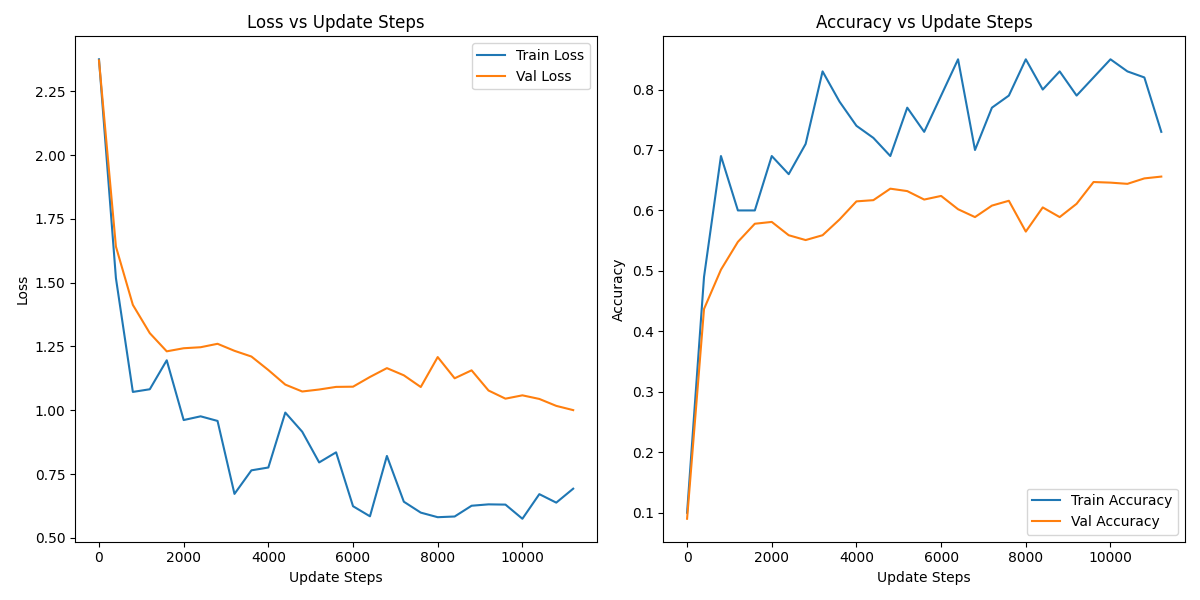
\includegraphics[width=0.75\textwidth]{results/architecture_updated_2_training_plot.png}
  \caption{Training and validation loss and accuracies for longer training runs for the updated Network Architecture 2 ($f=4, nf=40, nh=50$).}
  \label{fig:longer_training_runs_arch2_updated}
\end{figure}

The final test accuracies and training time for the above updated architecture after the longer training runs are as follows:
\begin{lstlisting}[caption={Final test accuracy and training time for updated Arch2 longer training runs}, label={lst:longer_training_runs_accuracies}]
Updated Network Arch2: Final test accuracy = 63.51% in training time of 58.46 seconds
\end{lstlisting}

We can see that increasing the layer width (number of filters) in the convolutional layer significantly decreases the loss and improves the final test accuracy, achieving a final test accuracy of 63.51\% compared to 57.35\% with the original architecture, also greater than the test accuracy of 60.38\% with the Network Architecture 3 ($f=8, nf=40, nh=50$). This is because smaller patches with the same number of filters lead to higher dimension feature representation, more detailed learning and in turn, better accuracy. 

I was able to verify the correctness of the above increased cyclic learning rate schedule with learning rate curve shown below:

\begin{figure}[H]
  \centering
  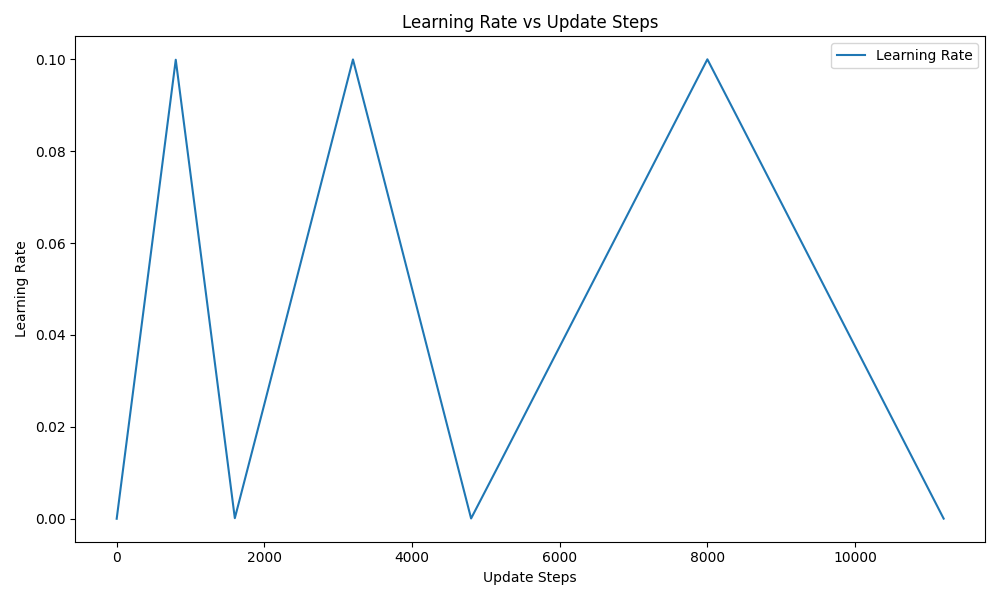
\includegraphics[width=0.6\textwidth]{results/architecture_4_learning_rate_plot.png}
  \caption{Increased Cyclic learning rate schedule for longer training runs.}
  \label{fig:increased_cyclic_learning_rate}
\end{figure}

\section*{Label Smoothing Vs No Label Smoothing}

We introduce a new Network Architecture 5 ($f=4, nf=40, nh=300$) with a larger fully connected layer and apply label smoothing to the output layer. The label smoothing is applied by modifying the target labels to be a mixture of the original one-hot encoded labels and a uniform distribution over all classes. The training runs are performed for 4 cycles with the same cyclic learning rate schedule as before, with $\lambda = 0.0025$. 
The training and validation curves for above run with and without label smoothing are shown below:
\begin{figure}[H]
  \centering
  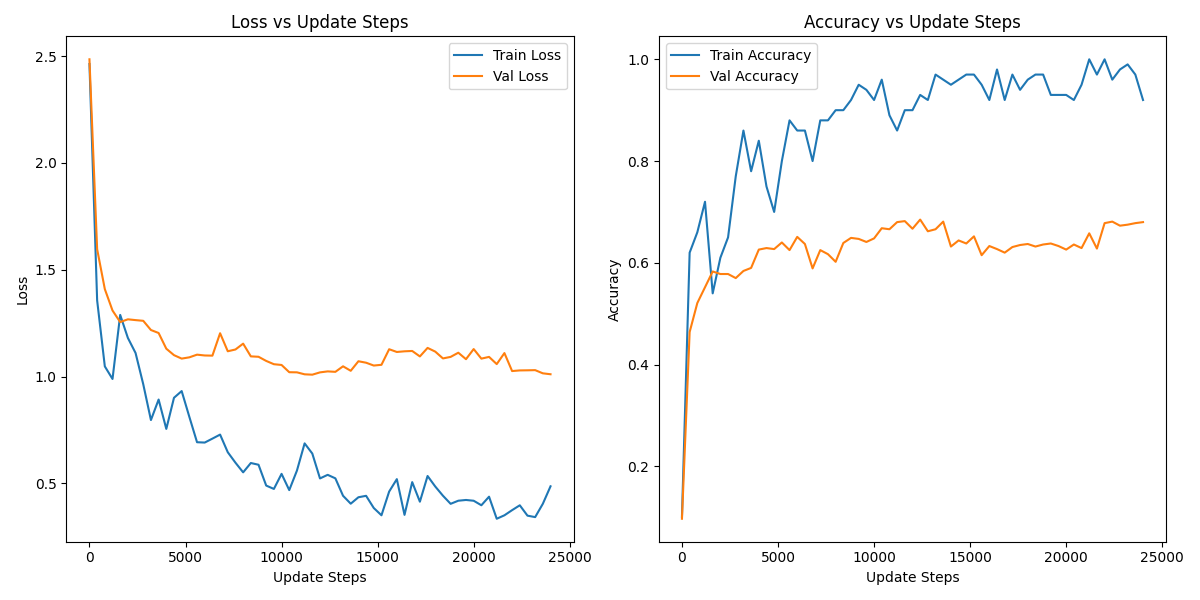
\includegraphics[width=0.75\textwidth]{results/architecture_ConvNet_smoothing_training_plot.png}
  \caption{Training and validation loss and accuracies for Network Architecture 5 ($f=4, nf=40, nh=300$) with label smoothing.}
  \label{fig:label_smoothing_arch5}
\end{figure}

\begin{figure}[H]
  \centering
  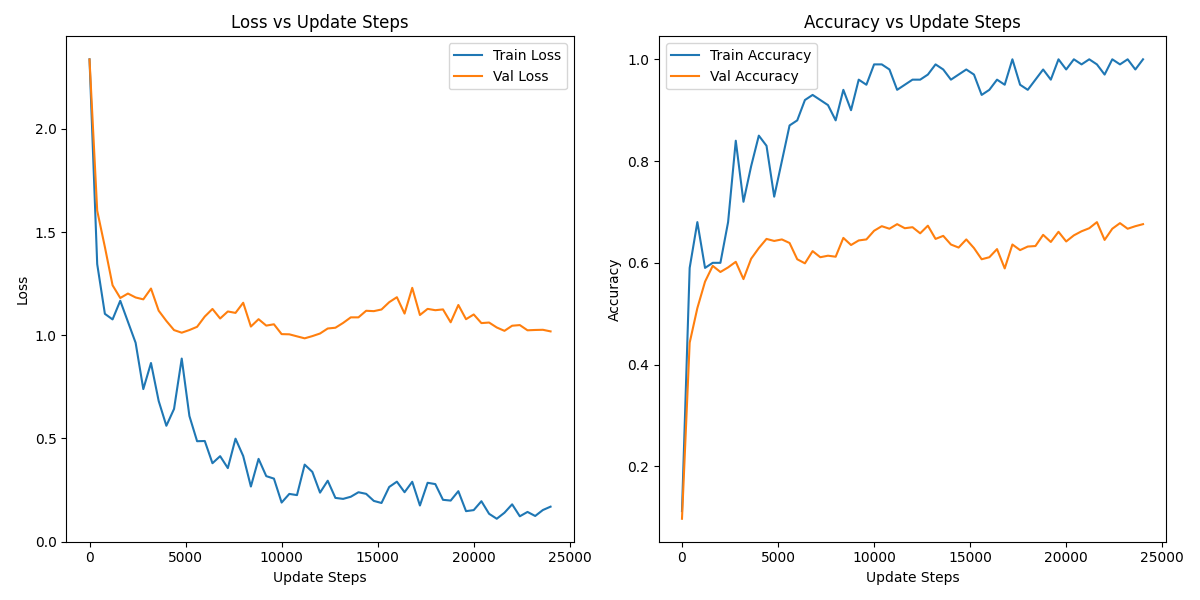
\includegraphics[width=0.75\textwidth]{results/architecture_ConvNet_no_smoothing_training_plot.png}
  \caption{Training and validation loss and accuracies for Network Architecture 5 ($f=4, nf=40, nh=300$) without label smoothing.}
  \label{fig:no_label_smoothing_arch5}
\end{figure}


The final test accuracies and training time for the above two architectures after the longer training runs are as follows:
\begin{lstlisting}[caption={Final test accuracies and training time of Arch5 with and without label smoothing}, label={lst:label_smoothing_accuracies}]
Arch5 with label smoothing: Final test accuracy = 66.05% in training time of 231.30 seconds
Arch5 without label smoothing: Final test accuracy = 65.96% in training time of 237.41 seconds
\end{lstlisting}




\end{document}